\documentclass[a4paper, 11pt]{article}

\usepackage{amsmath,amsfonts,amssymb,amsthm,graphicx,graphics,epsf}
\setcounter{tocdepth}{3}
\usepackage{graphicx}

\usepackage{algorithmic}
\usepackage{algorithm}
\usepackage{hyperref,color}
%\usepackage{comment}
%\usepackage{url}
\usepackage{xspace}
%\usepackage{lineno}
%\graphicspath{{img/}} % No need to write this for every figure
%\linenumbers


\usepackage{geometry}

\newtheorem{theorem}{Theorem}[section]
\newtheorem{corollary}[theorem]{Corollary}
\newtheorem{lemma}[theorem]{Lemma}
\newtheorem{proposition}[theorem]{Proposition}
\newtheorem{observation}[theorem]{Observation}
\newtheorem{problem}[theorem]{Problem}
\newtheorem{definition}[theorem]{Definition}
\newtheorem{conjecture}[theorem]{Conjecture}
\newtheorem{question}[theorem]{Question}



%%
%% Here you may place your macros using \newcommand{}{}
%%


\newcommand{\ve}{{\ensuremath{\vec{v}}}}   
\newcommand{\ue}{{\ensuremath{\vec{u}}}}  
\newcommand{\we}{{\ensuremath{w}}}    
  \newcommand{\red}{\color{red}}
  \newcommand{\cone}[1]{\ensuremath{\kappa_{\we}(#1)}}
  \newcommand{\ch}[1]{\ensuremath{\textsc{ch}(#1)}}
  \newcommand{\lt}{\ensuremath{ \leq_{\we}}}
    \newcommand{\ltc}{\ensuremath{ \leq_{-\we}}}
    \newcommand{\torus}{\ensuremath{\mathcal T}}


\newcommand{\C}[1]{\ensuremath{C_{\vec{#1}}}}
\newcommand{\A}[1]{\ensuremath{A_{\vec{#1}}}}



\begin{document}



\title{Triangulating with many tetrahedra}





\author{Luis Barba \and Jean Cardinal \and Stefan Langerman
}
\date{}

\maketitle
\begin{abstract}
Given a set of $n$ points in convex position in $\mathbb{R}^3$, we show that there exists a triangulation of this point set that consists of $\Omega(n \log\log n)$ tetrahedra.
\end{abstract}


%A category including the fourth, optional field follows..

\section{Outline}
\section{Preliminaries}
For any given integer $k$, let $Z_k = \{(x,y,z) \in \mathbb{R}^3 : z = k\}$.
Let $P = P_0\cup P_1$ be a set of $2n$ points in $\mathbb{R}^3$ such that $|P_0|= |P_1|$ and $P_i\subset Z_i$ for $i\in \{0, 1\}$.
Assume for ease of description that $P$ is in general position: 
no three points lie on a line and no two parallel lines contain more than one point. 

Let $S^k$ denote the unit sphere in dimension $k+1$.
Given a vector $\ue\in S^1$, its rotation matrix is defined as follows: 
$$M_\ue = \left[ \begin{array}{lr} \ue_x & -\ue_y \\ \ue_y & \ue_x \end{array} \right]\ ,$$
where $\ue_x$ and $\ue_y$ denote the $x$- and $y$-coordinates of $\ue$.

Recall that the surface of the unit torus, $\torus$, is equivalent to $\torus$, i.e., for each $\we\in \torus$, $\we = (\ve, \ue)$ where $\ve, \ue\in S^1$.

Given a point $\we = (\ve, \ue)$ on $\torus$, we use it to define a partial order on the points of $P_i$.
To this end, let $\ve_\ue = M_\ue (\ve)$ be the vector $\ve$ rotated by the angle given by $\ue$.
For each point $p\in P_i$, let $\cone{p} = \{ p  + \alpha \ve + \beta \ve_\ue \in Z_i : \alpha > 0, \beta \geq 0\}$ be the cone contained in $Z_i$ apexed at $p$. 
Note that since $\alpha$ is always greater than zero, the cone does not contain the ray shooting from $p$ in the direction of $\ue$; see Figure~\ref{fig:Cones}. (If $\ve = -\ue$, then $\cone{p}$ is the halfplane passing through $p$ with normal vector $M_{(0, -1)}(\ve)$, minus the ray shooting from $p$ in the direction of $\ue$).

Let $(P_i, \lt)$ be a partial order set (poset) defined as follows:
Given two points $p,q\in P_i$, we say that $p \lt q$ if and only if $q\in \cone{p}$.

\begin{figure}[tb]
\centering
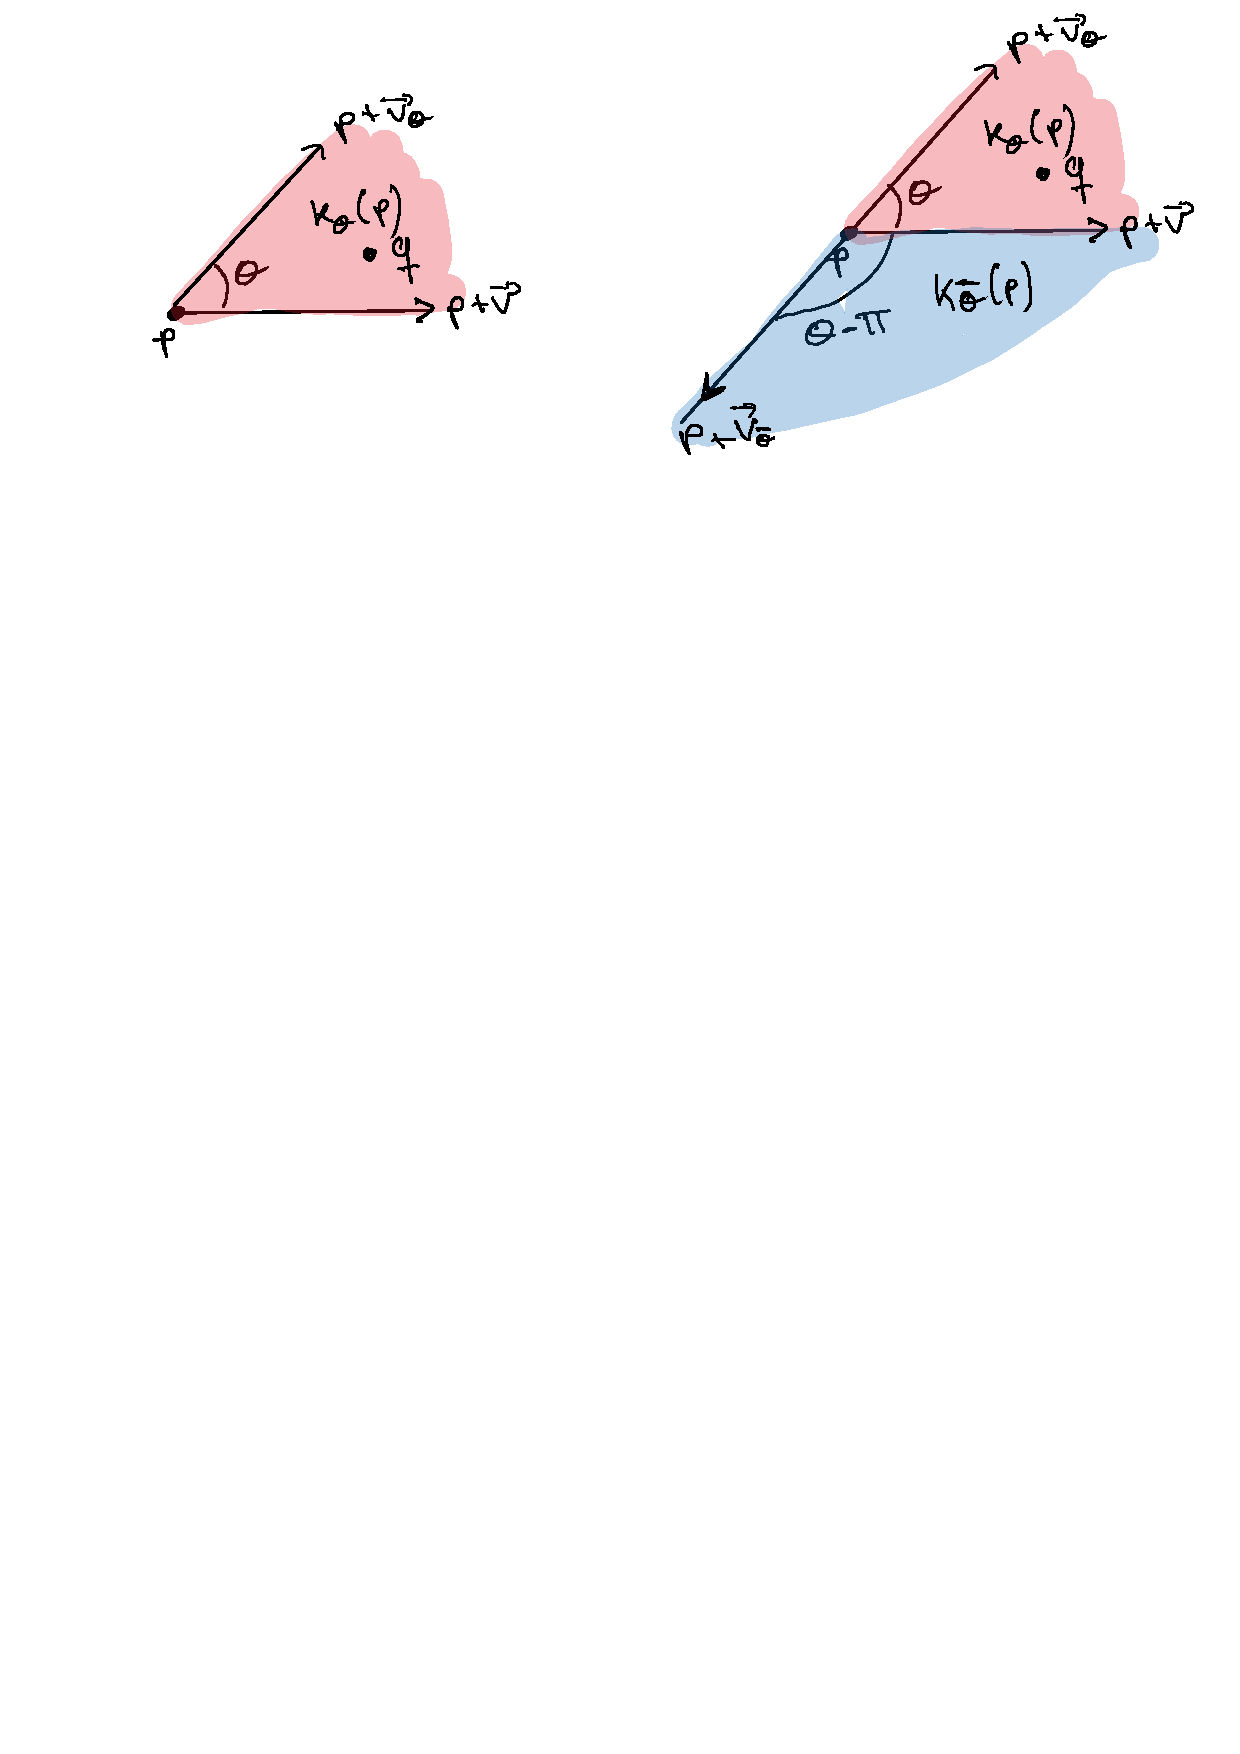
\includegraphics[width=1\textwidth]{img/Cones.pdf}
%[width=1\textwidth]
\caption{\small }
\label{fig:Cones}
\end{figure}

We say that two partial orders $(P_i, \leq')$ and $(P_i, \leq'')$ are \emph{complementary} if every two points of $P_i$ are comparable in $(P_i, \leq')\cup(P_i, \leq'')$ and only symmetric pairs (of the form $(p, p)$) are comparable in $(P_i, \leq')\cap(P_i, \leq'')$.

%Given $w = (\ve, \ue)$, let $\overline{\we} = (-\ve, \ue)$ be its \emph{mirroring}. 

\begin{lemma}\label{lemma:Properties of poset}
The posets $(P_i, \lt)$ and $(P_i, \ltc)$  are complementary.
\end{lemma}
\begin{proof}
Let $p$ and $q$ be two distinct points in $P_i$. 
%Notice that $q\in \cone{p}$ if and only if $p \in \kappa_{\overline{\we}}(q)$; see Figure~\ref{fig:Cones}. 
%Therefore, $p\lt q$ if and only if $p \leq_{\overline{\we}} q$ which shows that reversing $(P_i, \lt)$ yields the poset $(P_i, \leq_{\overline{\we}})$.
Assume without loss of generality that $\ve = (1,0)$ and that $p$ lies below $q$ in $P_i$.

Because $q$ lies above $p$, and since the union of $\cone{p}$ and $\kappa_{-\we}(p)$ contains all points with $y$-coordinate larger than $p$ in $P_i$, $q$ lies either in $\cone{p}$ or in $\kappa_{-\we}(p)$.
This implies that either $p\lt q$ or $p\ltc q$, but not both. 
Since $p$ and $q$ are arbitrary points, we conclude that any two points are either comparable in $(P_i, \lt)$ or in $(P_i, \ltc)$.
That is, $(P_i, \lt)$ and $(P_i, \ltc)$  are complementary.
\end{proof}

\subsection{Triangulation using chains and antichains}
Let $\we$ be a point on $\torus$.
Let $C = \{p_1, \ldots, p_k\}$ be a chain of $(P_0, \lt)$ and let $A = \{q_1, \ldots, q_t\}$ be  an antichain of $(P_1, \lt)$.
Recall that an antichain in $(P_1, \lt)$ is a chain in $(P_1, \ltc)$.
Assume without loss of generality that the elements of $C$ are sorted according to $\lt$ and that the elements of $A$ are sorted according to $\ltc$.
In this section, we show how to construct a triangulation of $C\cup A$ that has at least $|C|\cdot |A|$ tetrahedra.

To this end, we first construct a set of $|C|\cdot|A|$ tetrahedra that is a triangulation of a non necessarily convex polyhedra contained in $\ch{C\cup A}$. We then show how to extend this to a triangulation of $\ch{C\cup A}$ by gluing more tetrahedra.

Let $\varphi_0 = \cup\{p_j p_{j+1} : 1\leq j < k\}$ be the curve contained in $Z_0$, obtained by the union of the segments connecting consecutive elements of $A$. Define $\varphi_1 = \cup\{q_i  q_{i+1} : 1\leq i< t\}$ analogously.

For each $x\in \varphi_0$ and each $1\leq i < t$, let $\triangle_i(x) = \triangle(x, q_i, q_{i+1})$.
Let $\Pi_i(x)$ be the plane extending $\triangle_i(x)$ and let $\Pi^+_i(x)$ be the closed halfspace supported by $\Pi_i(x)$ that contains~$p_k$.

\begin{lemma}\label{lemma:Same side of plane}
For each $x,y\in \varphi_0$ such that $x\lt y\lt p_k$, it holds that $y\in \Pi_i^+(x)$. 
\end{lemma}
\begin{proof}
Let $\lambda$ be the line passing through $q_i$ and $q_{i+1}$ and let $\lambda_x$ be the line parallel to $\lambda$ passing through $x$. Thus, $\lambda_x\subset \Pi_i(x)$.

Because $q_i$ and $q_{i+1}$ are not comparable in $(P_1, \lt)$, both $x+\ve$ and $x+\ve_\ue$ lie on the same halfplane supported by $\lambda_x$ in $Z_0$, i.e., the cone $\cone{x}$ is contained in this halfplane. 
Because $p_k, y\in \cone{x}$ as $x\lt y\lt p_k$, and since $\Pi_i(x)$ contains $\lambda_x$, 
we conclude that $y\in \cone{x}\subset \Pi^+_i(x)$.
\end{proof}

Note that for any two points $x,y\in \varphi_0$ such that $y$ lies in the path contained in $\varphi_0$ connecting $x$ with $p_k$,
it holds that $x\lt, y\lt p_k$.

Let $S_x = \cup\{\triangle_i(x) : 1\leq i< t\}$ be the \emph{wavefront} at $x$.
Because all points in $A$ are coplanar, $S_x$ is a surface topologically equivalent to a disk; see Figure~\ref{fig:Wavefronts}.

\begin{figure}[tb]
\centering
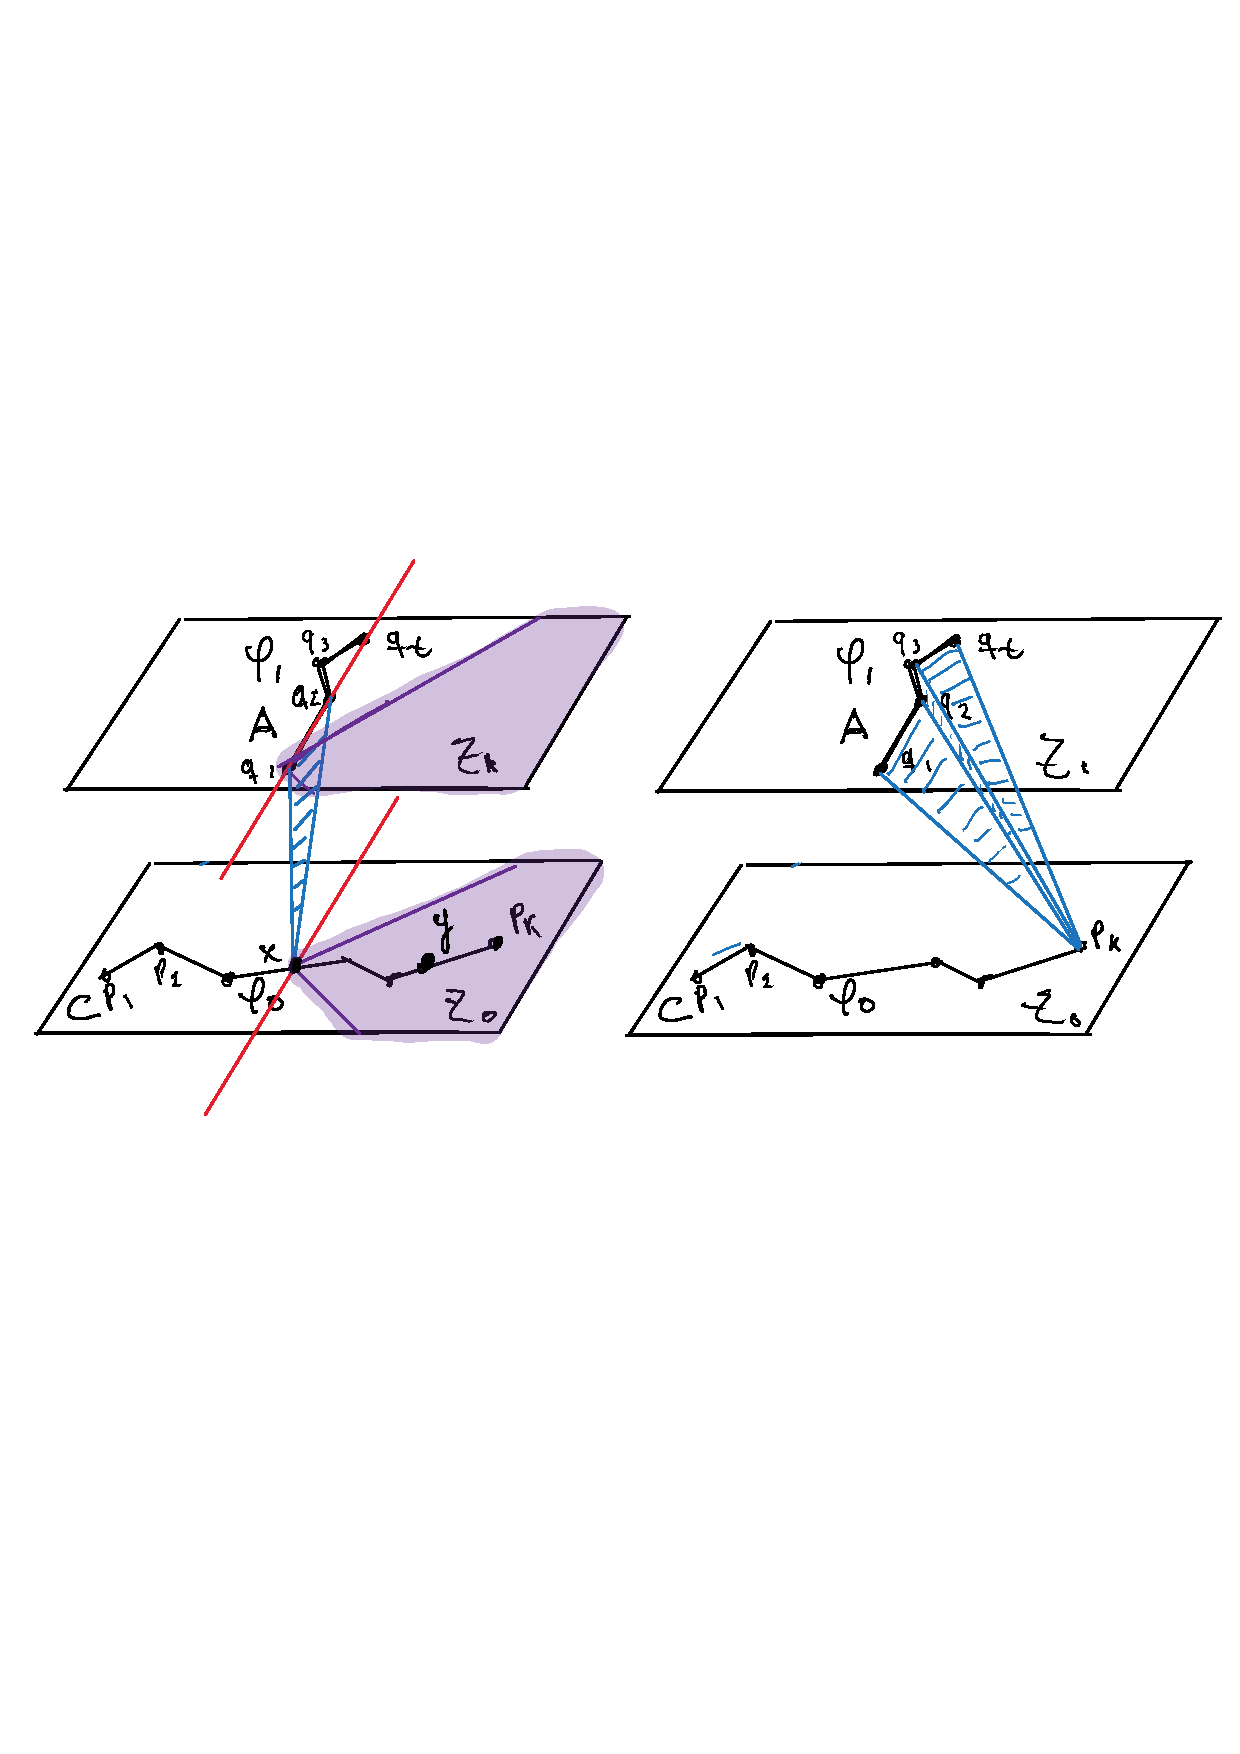
\includegraphics[width=1\textwidth]{img/Wavefronts.pdf}
\caption{\small }
\label{fig:Wavefronts}
\end{figure}

\begin{lemma}\label{lemma:Disjoint wavefronts}
For each $x, y\in \varphi_0$ such that $y$ lies in the path contained in $\varphi_0$ connecting $x$ with $p_k$,
it holds that $S_x\cap S_y = \varphi_1$.
\end{lemma}
\begin{proof}
Assume for a contradiction that there is a point $z\in \varphi_1$ such that the open segment $zy$ intersects $S_x$, i.e., $S_x$ and $S_y$ intersect.
Let $\triangle_i(x)$ be the first triangle intersected by $zy$ when going from $z$ towards $y$.
Because the segment $zy$ crosses the plane $\Pi_i(x)$, we conclude that $zy$ is not contained in $\Pi_i^+(x)$.

Assume that $z$ belongs to the segment $q_jq_{j+1}$ for some $1\leq j\leq t$. 
Thus, $z$ lies on the boundary of $\triangle_j(x)$. 
Let $R= \Pi^+_i(x)\cap \Pi^+_j(x)$  and note that $R$ is a convex set.
Because $y\in R$ by Lemma~\ref{lemma:Same side of plane} and since $z\in R$, we know that $zy\subset R$.
Since $R\subset \Pi_i^+(x)$, we conclude that $zy\subset \Pi_i^+(x)$---a contradiction. 
Therefore, for each $z\in \varphi_1$, the open segment $zy$ does not intersect $S_x$. 
Consequently, $S_x\cap S_y = \varphi_1$.
\end{proof}

To construct the triangulation, imagining moving $x$ continuously from $p_1$ to $p_k$ along $\varphi_0$ and taking the union of all wavefronts $S_x$. 
Let $T'$  be a set of $k\cdot t$ tetrahedra such that $$T' = \{\ch{p_i, p_{i+1}, q_j, q_{j+1}} : 1\leq i <k, 1\leq j < t\}.$$

\begin{lemma}\label{lemma:Interior disjoint tetrahedra}
The set $T'$ consists of interior disjoint tetrahedra whose union defines a simple polyhedron.
\end{lemma} 
\begin{proof}
Let $\sigma_{i,j} = \ch{p_i, p_{i+1}, q_j, q_{j+1}}$.
Assume for a contradiction that the interiors of $\sigma_{i,j}$ and $\sigma_{s,r}$ intersect for some $i,s \in \{1, \ldots, k\}$ and $j,r\in \{1, \ldots,  t\}$.
Therefore, the boundaries of $\sigma_{i,j}$ and $\sigma_{s,r}$ intersect at a point not on $\varphi_1$.
That is, a triangle $\triangle_j(x)$ intersects a segment $w y$ where $x\in p_ip_{i+1}, y\in p_s p_{s+1}$ and $w\in q_{r}q_{r+1}$.
Since $\triangle_j(x)\subset S_x$ and since $wy\subset S_y$,
this implies that the wavefronts $S_x$ and $S_y$ intersect---a contradiction with Lemma~\ref{lemma:Disjoint wavefronts}.
Therefore, $T'$ consists of interior disjoint tetrahedra.

To see that $\cup T'$ is a simple polyhedra, recall that $S_x$ is topologically equivalent to a disk for each $x\in \varphi_0$.
Notice that $\cup T' = \cup\{S_x : x\in \varphi_0\}$. Because each $S_x$ is disjoint, $\cup T'$ is topologically equivalent to a sphere, i.e., it is a simple polyhedra.
\end{proof}

By Lemmas~\ref{lemma:Interior disjoint tetrahedra}, we conclude that $T'$ is a triangulation of a simple polyhedron, say $\cup T'$, whose facets are triangles.

Our objective is to complete $T'$ to a triangulation $T$ of $\ch{C\cup A}$. To this end, we proceed as follows.
We say that two points are \emph{$T$-visible} if the open segment joining them does not intersect the interior of $\cup T$.
Let $\tau_i$ be a triangulation of $P_i$ in $Z_i$ such that $\gamma_i$ is contained in the union of the edges of $\tau_i$.
Notice that for each point $z\in \ch{C}$, either $q_1$ or $q_t$ is $T$-visible from $z$. 

In fact, the curve $\gamma_i$ splits $\ch{C}$ into two sets, the one containing the points visible from $q_1$ and the other containing those points visible from $q_t$.
This partition of $\ch{C}$ induces a partition of $\tau_1$ into two sets of the triangles, those visible from $q_1$ and those visible form $q_t$.
For each triangle $\triangle\in \tau_1$ visible from $q_1$ (\emph{resp.} $q_t$), we add the tetrahedron $\ch{\triangle, q_1}$ (\emph{resp.} $\ch{\triangle, q_t}$) to $T'$. 

In the same way, the triangulation $\tau_0$ can be partitioned into two sets of triangles, those visible from $p_1$ and those visible from $p_k$. We construct tetrahedra analogously for them and add them to $T'$.
In this manner, we obtain a new triangulation $T$ whose union is equal to $\ch{C\cup A}$; see Figure~\ref{fig:CompleteTriangulation} for an illustration.
Since the triangulation $T'$ has at least $|C|\cdot |A|$ tetrahedra and $T'\subseteq T$, $T$ consists of at least $|C|\cdot |A|$ tetrahedra.

\begin{figure}[tb]
\centering
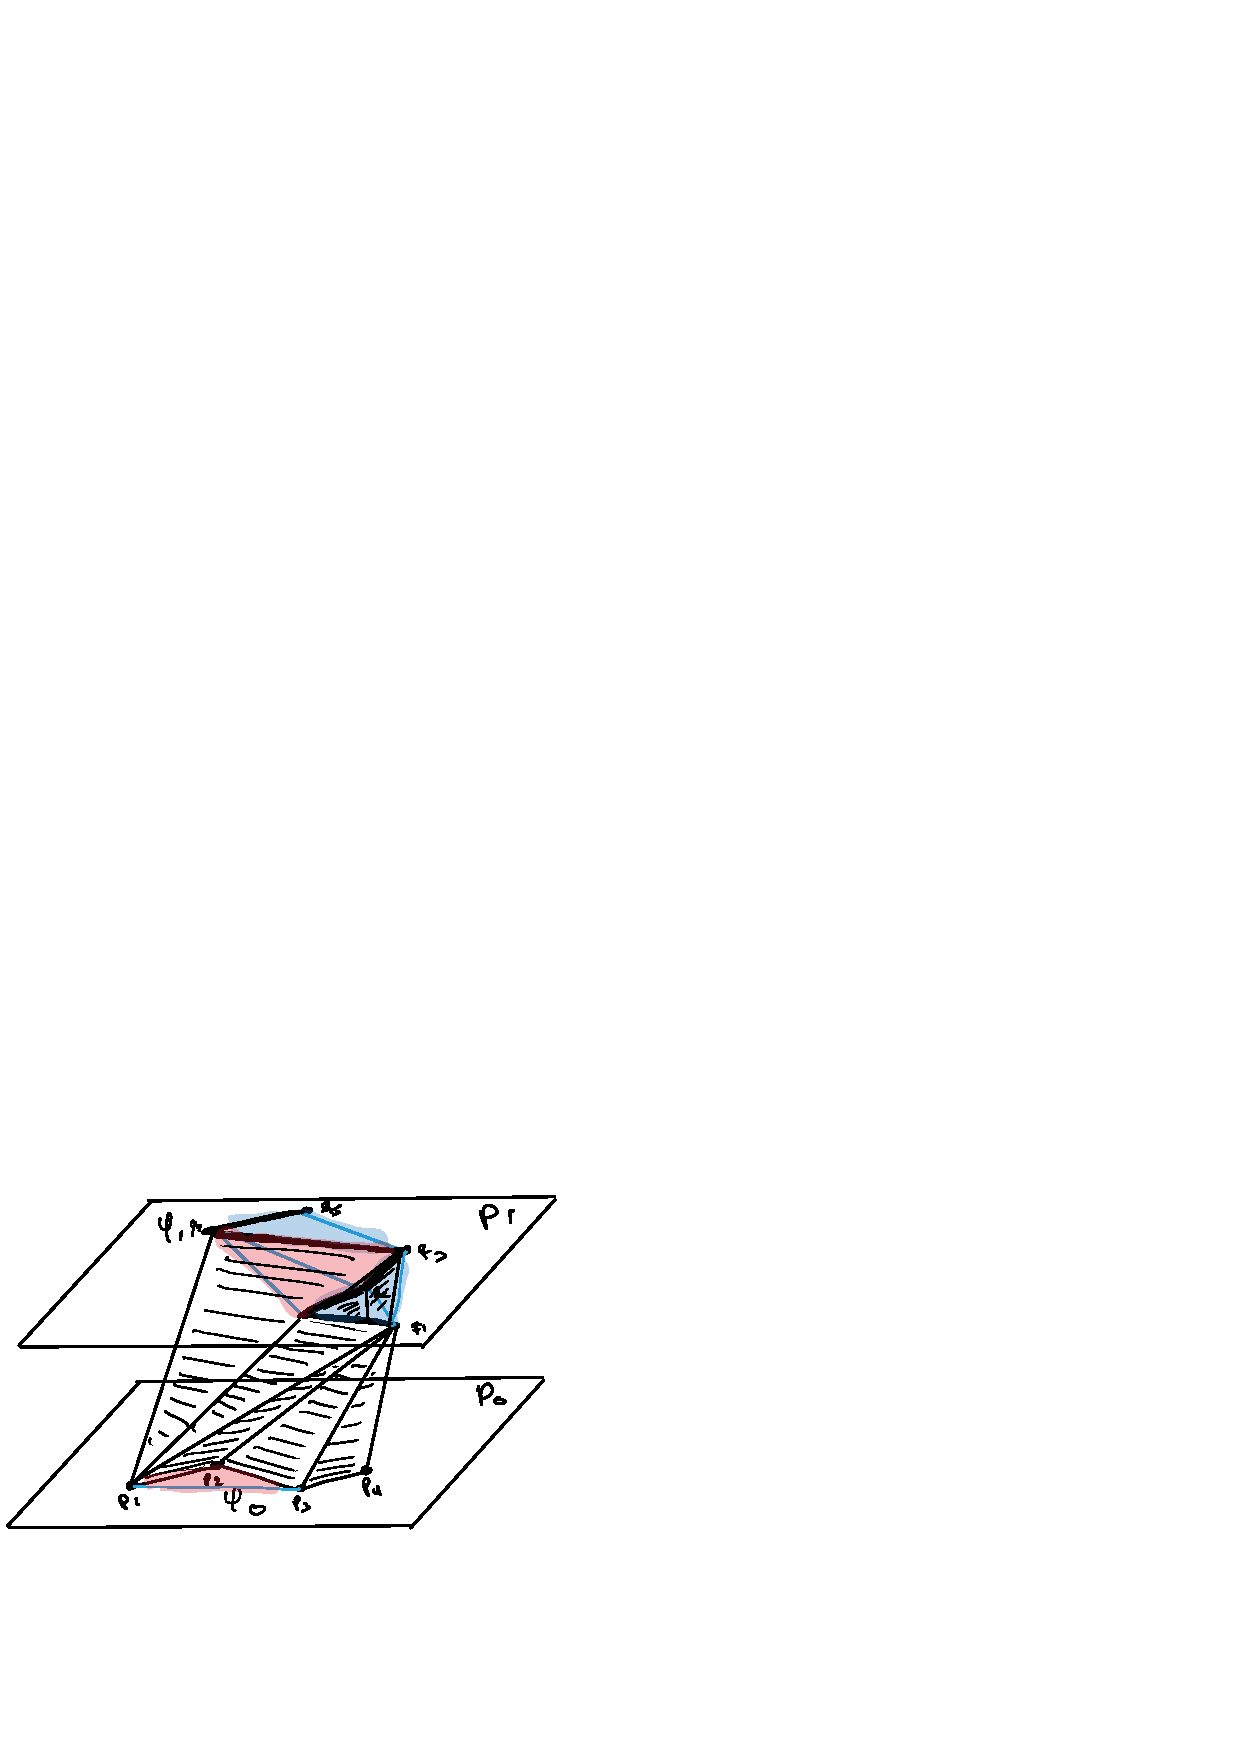
\includegraphics[width=1\textwidth]{img/CompleteTriangulation.pdf}
\caption{\small }
\label{fig:CompleteTriangulation}
\end{figure}
The following theorem summarizes the results presented in this section. 

\begin{theorem}\label{thm:Quadratic size Triangulation}
Give a chain $C$ of $(P_0, \lt)$ and  an antichain $A$ of $(P_1, \ltc)$,
there exists a triangulation of $\ch{C\cup A}$ that has at least $|C|\cdot |A|$ tetrahedra.
\end{theorem}


\subsection{Large chains and antichains}
For each $\we$ on $\torus$, Dilworth's theorem implies the existence of a chain $C^i_{\we}$ and an antichain $A^i_{\we}$ in $(P_i, \lt)$ such that  $|C^i_{\we}|\cdot |A^i_{\we}| \geq |P_i| = n$.
Assume that $C^i_{\we}$ and $A^i_{\we}$ are the lexicographically minimum subsets of $P_i$ with this property. 

Let $x(\we) = |C^0_{\we}| - |A^1_{\we}|$ and $y(\we) = |C^1_{\we}|- |A^0_{\we}|$.

\begin{lemma}\label{lemma:Properties of x}
For each $\we\in \torus$, it holds that \label{item:Antipodality} $x(\we) = -x(-\we)$.
%\begin{enumerate}
%\item  $x(\we) = x(\overline{\we})$.
%\item \label{item:Antipodality} $x(\we) = -x(-\we)$.
%\item $x(\ve, (1,0)) \in \{-n, 1-n\}$.
%\item $x(\ve, (-1,0)) \in \{n, n-1\}$.
%\end{enumerate}
\end{lemma}
\begin{proof}
%By Lemma~\ref{lemma:Properties of poset}, we know that $(P_i, \leq_{\overline{w}})$ is obtained by reversing $(P_i, \lt)$. Therefore, the sizes of the chains and antichains in these posets remain unchanged; property 1 follows.
By Lemma~\ref{lemma:Properties of poset} $(P_i, \lt)$ and $(P_i, \ltc)$ are complementary. 
This implies that any chain in $(P_i, \lt)$ is an antichain in $(P_i, \ltc)$ and viceversa. 
Therefore, the value of $x(\we) = -x(-\we)$.

%To prove property 3, notice that for each $p\in P_i$, the cone $\kappa_{(\ve, (1,0))}(p)$ consists of a single ray as $M_{(1,0)}$ is the identity matrix. Therefore, by our general position assumption, at most one point other than $p$ of $P_i$ lies on this ray, which implies that any chain in $(P_i, \leq_{\ve, (1,0)})$ has length at most two. 
%Since no two parallel lines contain more than one point by our general position assumption,  $x(\ve, (1,0))$ is equal to either $-n$ or $1-n$ yielding property 3. An analogous argument yields property 4.
\end{proof}

We say that a function $g:\mathbb{R}^m\to \mathbb{R}$ is \emph{almost continuous} if 
for any converging sequence $\{x_i\}_{i\in \mathbb{N}}$, there exists $n_0\in \mathbb{N}$ such that for any $i,j>n_0$, $|g(x_i) - g(x_j)|\leq 1$.

\begin{lemma}\label{lemma:Almost continuous}
The functions $x$ and $y$ are almost continuous.
\end{lemma}
\begin{proof}
Recall that $\we = (\ve, \ue)$, where $\ve,\ue\in S^1$.
If we fix the value of $\ue$, then by modifying the value of $\ve$, we obtain changes in $x(\we)$ only when a point stops (or starts) being inside a cone $\cone{p}$ for some $p\in P_i$ as it rotates around it. 
By the general position assumption of $P_i$, this change can increase or decrease the size of a chain (or antichain) by at most one.
Therefore, for a sufficiently small change in $\ve$, the value of $x(\we)$ changes by at most one.

If we fix the value of $\ve$, then by modifying the value of $\ue$, we change the aperture of the $\cone{p}$. 
In this case however, we have to be careful when $\ue$ reaches $(\cos(\pi), \sin(\pi))$.
Notice that the cone will point upwards for $(\cos(\pi-\varepsilon), \sin(\pi-\varepsilon))$ and downwards for $(\cos(\pi + \varepsilon), \sin(\pi+ \varepsilon))$. However, as $\varepsilon$ approaches zero, all the points will be comparable except for those lying in lines parallel to $\ve$. By our general position assumption, at most one line parallel to $\ve$ contains two points.
Therefore, $x(\we)$ is equal to either $n$ or $n-1$ when $\varepsilon$ reaches zero.
An analogous argument shows that for a fixed value of $\ue$, 
any sufficiently small change in $\ve$ produces a change in $x(\we)$ of at most one. 

Consequently, for any converging sequence $\{\we_i\}_{i\in \mathbb{N}}$ in $\torus$, 
there exists $n_0$ such that for any $i,j>n_0$, $|x(\we_i) - x(\we_j)| \leq 1$. 


The same argument holds for the function~$y$.
\end{proof}


\begin{lemma}\label{lemma:Similar function}
There exist continuous functions $g_x, g_y:\torus\to \mathbb{R}$ such that for any $\we\in \torus$, it holds that  $| x(\we) - g_x(\we) | \leq 1$ and $| y(\we) - g_y(\we) |\leq 1$.
\end{lemma}
\begin{proof}
Because discontinuities in $x$ arise only when the boundary of a cone $\cone{p}$ passes through a second point, function $x$ has a set of discontinuities of measure zero. Therefore, $x$ is a Baire class one-function~\cite{?}, i.e., it can be defined as the pointwise limit of continuous functions. Thus, there exist a function $g_x:\torus \to \mathbb{R}$ such that $| x(\we) - g_x(\we) | \leq 1$ for all $\we\in \torus$. An analogous proof applies for $y$.
\end{proof}



\begin{lemma}
There exists $\we^*\in \torus$ and an integer $i\in \{0, 1\}$ such that 
$|C^i_{\we^*}| \cdot |A^{1-i}_{\we^*}| \geq n$, and both $C^i_{\we^*}$ and $A^{1-i}_{\we^*}$ have size  at least $\sqrt{n}-1$.
\end{lemma}
\begin{proof}
Because $g_x$ is a continuous function from the torus $\torus$ to $\mathbb{R}$ by Lemma~\ref{lemma:Similar function}, the Borsuk-Ulam theorem~\cite{?} implies the existence of a point $\we^*$ such that $g_x(\we^*) = g_x(-\we^*)$, i.e., two antipodal points with the same value.
Thus, Lemma~\ref{lemma:Similar function} implies that $|x(\we^*) - x(-\we^*)| \leq 2$. 
Because $x(\we^*) = - x(-\we^*)$ by Lemma~\ref{lemma:Properties of x}, 
we get that $|x(\we^*) + x(\we^*)| \leq 2$, which implies that $|x(\we^*)|\leq 1$. Consequently $-1\leq x(\we^*) = |C^0_{\we^*}| - |A^1_{\we^*}| \leq 1$, i.e., the sizes of $C^0_{\we^*}$ and $A^1_{\we^*}$ differ at most by one.
If $\max\{|C^0_{\we^*}|, |A^1_{\we^*}|)\} \geq \sqrt{n}$, then our result follows. Otherwise, we can assume that 
\begin{equation}\label{eq:Assumption size}
\max\{|C^0_{\we^*}|, |A^1_{\we^*}|)\} < \sqrt{n}.
\end{equation}



Note that by definition $|C^i_{\we^*}| \cdot |A^i_{\we^*}| \geq n$ for $i\in \{0, 1\}$. 
Therefore, by (\ref{eq:Assumption size}) we know that $|C^1_{\we^*}| > \sqrt{n}$ and $|A^0_{\we^*}| > \sqrt{n}$.
Moreover, we have 
$$(|C^0_{\we^*}|\cdot |A^1_{\we^*}|) (|C^1_{\we^*}|\cdot |A^0_{\we^*}|) \geq n^2.$$
Because $\max\{|C^0_{\we^*}|, |A^1_{\we^*}|)\} < \sqrt{n}$ by (\ref{eq:Assumption size}), $|C^0_{\we^*}|\cdot |A^1_{\we^*}| < n$. 
Consequently, $|C^1_{\we^*}|\cdot |A^0_{\we^*}| > n$ proving our result.
\end{proof}

\begin{corollary}\label{corollary:Existence of set}
There exists a set $S$ of $2\sqrt{n}-2$ points of $P$ such that $\ch{S}$ has a triangulation with $\Theta(n)$ tetrahedra.
\end{corollary}

\subsection{Constructing complete triangulations}
Let $S$ be the set of $2\sqrt{n}-2$ points of $P$ given by Corollary~\ref{corollary:Existence of set} having a triangulation with $\Theta(n)$ tetrahedra.
To extend this triangulation of $S$ to a triangulation of $P$, we proceed recursively. Let $\Sigma = \{\sigma_1, \ldots, \sigma_k\}$ be the set of planes that extend all the facets of $\ch{S}$. Because $|S| = \Theta(\sqrt{n})$, we know that $k =  O(\sqrt{n})$ (it could be that many triangles are coplanar in either $P_0$ or $P_1$).
We construct $k$ sets $P^1, \ldots P^k$ as follows: 
Let $P^i$ be the set of remaining points of $P$ that lie on the halfspace supported by $\sigma_i$ that does not contain $\ch{S}$.
Remove $P^i$ from $P$ and continue the proceed recursively with~$i+1$.
As a \emph{separation invariant}, note that $\sigma_i$ separates $P_i$ from $S$ and from the remaining points of $P$.

Since the convex hulls of the $P^i$s are pairwise disjoint, we can proceed recursively and obtain a triangulation of their convex hull. 
To complete the process, we merge the convex hull $S$ with the convex hulls of the $P^i$s in reverse order. 
That is, we first merge $\ch{S}$ with $\ch{P^k}$, then the resulting convex hull with $\ch{P_{k-1}}$ and so on. 
We claim that this merge is always possible. 

To prove this claim, let $S_0 = S$, and let $S_j = S\cup (\cup_{i=0}^{j -1} P^{k-i})$ for each $1\leq j\leq k$. 
Notice that by the separation invariant, for each $1\leq  j \leq k$, the plane $\sigma_j$ separates $\ch{S_{j-1}}$ from $\ch{P_j}$.
Therefore, for each $1\leq i < j \leq k$, $\ch{P_i}$ cannot intersect $\ch{S_j}$. Otherwise, $\sigma_i$ does not separate $\ch{P_i}$ from $\ch{S_{i-1}}$. Therefore, the recursive process ends with a triangulation of $\ch{S_k} = \ch{P}$.

It remains only to analyze the size of this triangulation. To this end, recall that the triangulation of $S$ contains $\Theta(n)$ triangles.
Moreover, since $k = O(n)$, at least one of the $P^i$s has $\Omega(\sqrt{n})$ points.
We obtain the following recurrence $T(n) = \sum_{i=1}^k T(n_i) + \Omega(n)$, where $k = O(\sqrt{n})$ (and hence some $n_i = \Omega (\sqrt{n})$). 
By induction, we can show that $T(n) = \Omega(n\log\log n)$.



\end{document}  